%  !TeX  root  =  user_guide.tex

\chapter{Utilisation des extensions principales de \qg}\label{sec:core_plugins}\index{extensions!principales}

\qg \CURRENT contient 22 extensions principales qui peuvent être chargées depuis le Gestionnaire d'Extensions.

{\setlength{\extrarowheight}{15pt}
\small
\begin{longtable}{|p{1cm}|p{4cm}|p{8cm}|p{3cm}|}
\caption{26 Extensions principales de QGIS}\label{tab:core_plugins} \\
\hline
  \textbf{Icône} & \textbf{Extension} & \textbf{Description} & \textbf{Référence du manuel}\\
\endfirsthead
\hline 
  \textbf{Icône} & \textbf{Extension} & \textbf{Description} & \textbf{Référence du manuel}\\
\endhead
\hline 

\includegraphics[width=0.6cm]{delimited_text}
 & Ajouter une couche texte délimité \index{extensions!texte delimite} & Charger et afficher des fichiers texte délimité contenant des coordonnées x et y & Chapter \ref{label_dltext}\\
\hline

\includegraphics[width=0.6cm]{coordinate_capture}
 & Saisie de coordonnées \index{extensions!saisie de coordonnees} & Capturer les coordonnées de la souris dans différents SCR & Chapter \ref{coordcapt}\\
\hline 

\includegraphics[width=0.6cm]{copyright_label}
 & Etiquette de copyright \index{extensions!copyright} & Afficher une étiquette de copyright avec les informations associées & Chapter \ref{copyrightlabel}\\
\hline

\includegraphics[width=0.6cm]{plugin}
 & Diagramme de couche \index{extensions!diagram} & Placer des graphiques (camemberts, barres) ou des symboles proportionnels sur des couches vectorielles & Chapter \ref{sec:diagram}\\
\hline

\includegraphics[width=0.6cm]{plugin}
 & Déplacement \index{plugins!point displacement}& Ajoute un nouveau moteur de rendu qui gère le déplacement de point automatiquement lorsque ils se superposent & Chapter \ref{new_generation_sym}\\
\hline
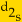
\includegraphics[width=0.6cm]{dxf2shp_converter}
 & Convertisseur DXF2Shape \index{extensions!DXF2Shape} & Convertir un fichier au format DXF vers le format SHP & Chapter \ref{dxf2shape}\\
\hline
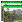
\includegraphics[width=0.6cm]{evis_icon}
 & eVis & Outil de Visualisation d'Événements\\
\hline

\includegraphics[width=0.6cm, height=0.6cm]{ftools_logo}
 & fTools \index{extensions!ftools} & Une suite d'outils de recherche, d'analyse, de géométrie et de géotraitement & Chapter \ref{sec:ftools}\\
\hline

\includegraphics[width=0.6cm]{gps_importer}
 & Outils GPS \index{extensions!gps} & Charger et importer des données GPS & Chapter \ref{label_plugingps}\\
\hline

\includegraphics[width=0.6cm]{grass}
 & GRASS \index{extensions!\grass!boîte à outils} & Activer la puissante boîte à outils GRASS & Chapter \ref{sec:grass}\\
\hline

\includegraphics[width=0.6cm, height=0.6cm]{raster-info}
 & Outils GDAL \index{extensions!gdaltools} & Une interface graphique simplifiée pour les programmes de traitement raster GDAL & Chapitre \ref{label_plugingdaltools}\\
\hline

\includegraphics[width=0.6cm]{georeferencer}
 & Géoréférencer \index{extensions!géoréférencement} & Ajouter des informations de projection aux fichiers raster & Chapitre \ref{sec:georef}\\
\hline

\includegraphics[width=0.6cm]{interpolation}
& Interpolation \index{extensions!Interpolation} & Interpolation sur la base de sommets d'une couche vectorielle & Chapitre \ref{sec:interpol}\\
\hline

\includegraphics[width=0.6cm]{mapserver_export}
& Export MapServer \index{extensions!export MapServer} & Exporter un projet \qg au format mapfile de MapServer &  Chapitre \ref{sec:mapserver_export}\\
\hline

\includegraphics[width=0.6cm]{north_arrow}
& Flèche Nord \index{extensions!north arrow} & Afficher une rose des vents au premier plan de la carte & Chapter \ref{northarrow}\\
\hline

\includegraphics[width=0.6cm]{offline_editing_copy}
 & Édition offline & Édition offline et synchronisation avec une base de données & Chapitre \ref{sec:offlinedit}\\
\hline
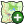
\includegraphics[width=0.6cm]{osm_load}
 & OpenStreetMap & Visualiser et éditer des données OpenStreetMap & Chapitre \ref{plugins_osm}\\
\hline

\includegraphics[width=0.6cm]{oracle_raster}
 & Georaster Oracle \index{extensions!georaster} & Accéder à des géorasters Oracle Spatial & Chapitre \ref{sec:oracleraster}\\
\hline
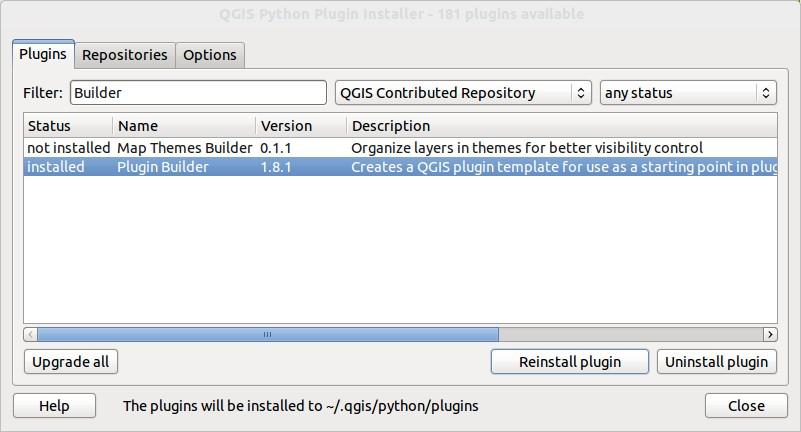
\includegraphics[width=0.6cm]{plugin_installer}
 & Installateur d'extensions \index{extensions!installation} & Télécharger et installer des extensions Python & Chapitre \ref{sec:python_plugin_installer}\\
\hline

\includegraphics[width=0.6cm]{raster_terrain}
 & Modelisateur de terrain \index{extensions!Raster Terrain Modelling} & Calculer la pente, l'aspect et la courbure totale des MNT & Chapitre \ref{sec:rasterrain}\\
\hline

\includegraphics[width=0.6cm]{plugin}
 & Graphique routier \index{plugins!road graph} & Résoud le problème du plus court chemin & Chapter \ref{sec:roadgraph} \\
\hline

\includegraphics[width=0.6cm]{spiticon}
 & SPIT \index{extensions!spit} & Outil d'import de fichiers Shape vers PostgreSQL/PostGIS & Chapitre \ref{sec:loading_postgis_data}\\
\hline

\includegraphics[width=0.6cm]{plugin}
 & SQL anywhere \index{plugins!SQL anywhere} &  Store des couches vecteurs dans une base de données SQL anywhere & Chapitre \ref{sec:sqlanywhere} \\
\hline

\includegraphics[width=0.6cm]{scale_bar}
 & Barre d'échelle \index{extensions!barre d'échelle} & Afficher une barre d'échelle au premier plan de la carte & Chapitre \ref{scalebar}\\
\hline

\includegraphics[width=0.6cm]{spatialquery}
 & Requête spatiale & Réalise des requêtes spatiales sur des couches vecteurs & Chapter \ref{sec:spatial_query} \\
\hline

\includegraphics[width=0.6cm]{mIconAddWfsLayer}
 & WFS & Charger et afficher une couche WFS & Chapitre \ref{sec:ogc-wfs}\\
\hline
\end{longtable}}

